\chapter{Modellbeschreibung}
Das verwendete Modell kann durch folgende Lattice Boltzmann Gleichung beschrieben werden \cite{Leclaire2011}:
\begin{equation}
N_i^k(\vec{x} + \vec{c_i} \delta t, t+\delta t) = N_i^k(\vec{x},t) + \Omega_i^k \left( N_i^k(\vec{x},t) \right).
\end{equation}

Der Kollisionsoperator ist dabei aus verschiedenen Operatoren zusammengesetzt:
\begin{equation}
 \Omega_i^k  \left( N_i^k(\vec{x},t)\right) = (\Omega_i^k)^{(3)} \left[ (\Omega_i^k)^{(1)} + (\Omega_i^k)^{(2)} \right] \left( N_i^k(\vec{x},t)\right). 
\end{equation}

Die einzelnen Operatoren werden im folgenden kurz beschrieben.

\section{Single phase collision (BGK)}
Der erste Sub-Operator ist im Kern der klassische BGK-Operator:
\begin{equation}
 (\Omega_i^k)^{(1)} (N_i^k) = N_i^k - \omega \left(N_i^k - {N_i^k}^{(e)} \right)
\end{equation}
Als Gleichgewichts-Funktion wird folgende verwendet \cite{Reis2007}:
\begin{equation}
\label{eq:equilibrium}
 {N_i^k}^{(e)} = \rho_k \left( \phi_i^k + w_i \left[3 \vec{c_i} \cdot \vec{u} + \frac{9}{2} (\vec{c_i} \cdot \vec{u})^2 - \frac{3}{2} (u^2) \right]  \right)
\end{equation}
mit $\rho_k = \sum_i N_i^k$, $ \rho u = \sum_i \sum_k N_i^k c_i$ und $\rho = \sum_k \rho_k$ sowie den Wichtungsfaktoren:
\begin{equation}
 w_i = \left\lbrace \begin{array}{ll} 4/9 &i = 1 \\ 1/9 & i= 2,4,6,8 \\ 1/36 & i = 3,5,7,9  \end{array}     \right. .
\end{equation}
Außerdem:
\begin{equation}
 \phi_i = \left\lbrace \begin{array}{ll} \alpha_k &i = 1 \\ (1-\alpha_k)/5 & i= 2,4,6,8 \\ (1-\alpha_k)/20 & i = 3,5,7,9  \end{array}     \right. .
\end{equation}
Um eine stabile Grenzfläche zu erhalten wird das Dichte-Verhältnis eingeführt \cite{Grunau1993,Reis2007,Leclaire2011}:
\begin{equation}
 \gamma = \frac{\rho_r}{\rho_b} = \frac{1 - \alpha_b}{1 - \alpha_r}
\end{equation}
Der Druck kann beschrieben werden durch:
\begin{equation}
 p_k = \frac{3 \rho_k (1- \alpha_k)}{5}= \rho_k (c_s^k)^2
\end{equation}
Somit ist $\alpha_k$ ein Maß für die Schallgeschwindigkeit im Fluid $k$. Damit ist entweder $\alpha_b$ oder $\alpha_r$ ein freier Parameter.
Leclaire et al. haben für das System Luft-Wasser $\alpha_b = \num{0.2}$ gesetzt \cite{Leclaire2011}. Damit ergibt sich für $\alpha_r$:
\begin{align}
 \frac{\rho_r}{\rho_b} &= \frac{1 - \alpha_b}{1 - \alpha_r} \\
(1 - \alpha_r) \rho_r & =  (1 - \alpha_b) \rho_b \\
(1 - \alpha_r) &= \frac{ (1 - \alpha_b) \rho_b}{\rho_r} \\
\alpha_r &= 1 - \frac{ (1 - \alpha_b) \rho_b}{\rho_r}
\end{align}
Allerdings wird weder bei \cite{Reis2007} noch bei \cite{Leclaire2011} klar, ob diese Rechnung nur einmal zu Beginn der Simulation mit festem $\gamma$ oder während der Simulation in jeder Zelle erfolgt. 
Da versuche mit einer Berechnung in jeder Zelle fehlschlugen -- bei sehr kleinem $\rho_r$ geht $\alpha_r$ gegen $- \infty$ und die Massenerhaltung wird verletzt -- wird davon ausgegangen, dass die Berechnung bei festem $\gamma$ zu erfolgen hat:
\begin{equation}
 \alpha_r = 1 - \frac{1 - \alpha_b}{\gamma}.
\end{equation}


Der Relaxationsparameter wird abhängig von $\psi$:
\begin{equation}
 \psi = \frac{\rho_r - \rho_b}{\rho_r + \rho_b},
\end{equation}
 entweder als $\omega_r$ oder $\omega_b$ oder als Interpolation zwischen beiden angenommen:
\begin{equation}
 \omega(\psi) = \left\lbrace 
\begin{array}{ll}
  \omega_r & \psi > \delta \\
  f_r(\psi) &   0 < \psi \leq \delta \\
  f_b(\psi) & -\delta \leq \psi \leq 0 \\
  \omega_b & \psi < -\delta
\end{array} \right. ,
\end{equation}
mit:
\begin{align}
 f_r(\psi) &= \chi + \eta \psi + \kappa \psi^2 , \\
 f_b(\psi) &= \chi + \lambda \psi + \nu \psi^2 .
\end{align}
Die hier auftretenden Parameter sind definiert als:
\begin{align}
 \chi &= 2 \omega_r \omega_b / (\omega_r + \omega_b) \\
 \eta &= 2(\omega_r - \chi)/\delta \\
 \kappa &= -\eta / (2 \delta) \\
 \lambda &= 2(\chi - \omega_b) / \delta \\
 \nu &= \lambda / (2 \delta)
\end{align}

Bei Leclaire et al.  wurden die Viskositäten noch nicht variiert, weshalb $\omega_r = \omega_b = 1$ ist und $\delta = 0,1$ keinen Einfluss auf das Ergebnis hat. 
Die Viskositätsunterschiede wurden von Leclaire et al. erst später eingebracht \cite{Leclaire2012}.

\subsection{Einbau von Gravitation}
Der Einfluss der Schwerkraft kann als zusätzlicher \emph{forcing term} in das Modell eingearbeitet werden \cite{Guo2002}: 
\begin{equation}
 (\Omega_i^k)^{(1)} (N_i^k) = N_i^k - \omega \left(N_i^k - {N_i^k}^{(e)} \right) + G_i \delta t.
\end{equation}
mit 
\begin{equation}
 G_i = \left( 1 - \frac{1}{2} \omega  \right) \cdot w_i \left[ (\vec{c_i} - \vec{u})  + (\vec{c_i} \cdot \vec{u}) \vec{c_i}   \right] \cdot \vec{G}
\end{equation}
$\vec{G}$ ist dabei der Kraftvektor einer externen Kraft. 
\subsubsection{Probleme}
Zunächst wurde versucht ein allgemeiner Ansatz zu implementieren. Dabei war $\vec{G}$ die nach unten gerichtete Schwerkraft:
\begin{equation}
 \vec{G} = \left( \begin{array}{c} 
                   0 \\
		  - \rho \cdot V \cdot g
                  \end{array} \right) .
\end{equation}
mit konstantem $V$. 
Die Idee war, dass das dichtere Medium stärker nach unten gezogen wird als das dünnere und somit dieses nach oben drückt. 
Allerdings wird die Grenzfläche instabil, wenn der Dichtegradient in der kontinuierlichen Phase zu groß wird. 
Alternativ wird direkt eine Auftriebskraft auf die Gas-Phase aufgeprägt:
\begin{equation}
 \vec{G} = \left( \begin{array}{c} 
                   0 \\
		  + (\rho_l - \rho_g) \cdot V \cdot g
                  \end{array} \right) .
\end{equation}
In diesem Ansatz ist $\rho_l$ konstant und $\rho_g$ wird aus den Dichteverteilungen gewonnen.


In der Implementierung wird nicht der BGK-Ansatz verwendet sondern ein MRT-Ansatz. Genaueres dazu in \autoref{chap:MRT}.

\section{Perturbation}
Der zweite Operator bewirkt eine Separation entlang des Farb-Gradienten:
\begin{equation}
 (\Omega_i^k)^{(2)} (N_i^k) = N_i^k + \frac{A_k}{2} \left| \vec{F} \right| \left[w_i \frac{(\vec{F} \cdot \vec{c_i})^2 }{\left| \vec{F} \right|^2} -B_i  \right]
\end{equation}
Der Parameter $A_k$ bestimmt die Stärke dieser Trennung und kann somit als Maß für die Oberflächenspannung genutzt werden \cite{Gunstensen1991}. Der Wert von $B_i$ wird so gewählt, dass die Chapman-Enskrog-Erweiterung die klassischen Navier-Stokes-Gleichungen ergibt \cite{Reis2007}:
\begin{equation}
 B_i = \left\lbrace 
\begin{array}{ll}
- 4/27 & i = 1 \\
2/27 & i = 2,4,6,8 \\
5/108 & i= 3,5,7,9
\end{array} \right.
\end{equation}
Der Farb-Gradient $\vec{F}$ kann definiert werden als der Gradient des Farbunterschiedes $\Delta(\vec{x}) = \rho_r(\vec{x}) - \rho_b(\vec{x})$:
\begin{equation}
 \vec{F} = \nabla (\rho_r(\vec{x}) - \rho_b(\vec{x}))
\end{equation}
Dieser Gradient kann angenähert werden durch \cite{Grunau1993,Reis2007}:
\begin{equation}
 \vec{F}(\vec{x}) = \sum_i \vec{e_i} \Delta(\vec{x} + \vec{e_i}) 
\end{equation}
Diese anisotrope Näherung führt bei großen Dichteverhältnissen zu Problemen und wird deshalb durch eine Wichtung der einzelnen Summanden isotrop bis auf einen räumlichen Fehler 4. Ordnung angenähert \cite{Leclaire2011}.
Dazu müssen die Dichteunterschiede in 4 weiteren Zellen berücksichtigt werden.

\begin{figure}
\centering
 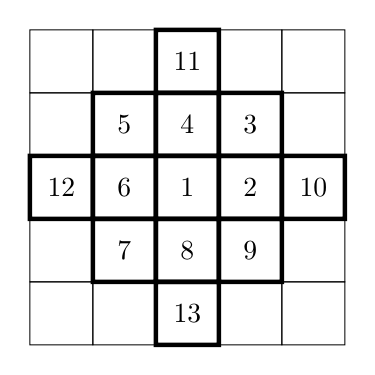
\begin{tikzpicture}
\def\scale{0.4}

\def\root{1.41421356 * \scale}

\def\quad#1#2{
  \draw[ultra thick] #1 #2 +(0:\scale) \foreach \a in {45,135,225,315} { -- +(\a:\root) } -- cycle;
}
\def\quadt#1#2{
  \draw #1 #2 +(0:\scale) \foreach \a in {45,135,225,315} { -- +(\a:\root) } -- cycle;
}


% Draw grid of small squares

\foreach \a in {-\scale,0,\scale} {\quad{ (0,0)}{(2*\a,2*\scale)}}
\foreach \a in {-\scale,0,\scale} {\quad{ (0,0)}{(2*\a,0)}}
\foreach \a in {-\scale,0,\scale} {\quad{ (0,0)}{(2*\a,-2*\scale)}}

\foreach \a in {-2*\scale,-1*\scale,0,1*\scale,2*\scale} {\quadt{ (0,0)}{(2*\a,-4*\scale)}}
\foreach \a in {-2*\scale,-1*\scale,0,1*\scale,2*\scale} {\quadt{ (0,0)}{(2*\a,-2*\scale)}}
\foreach \a in {-2*\scale,-1*\scale,0,1*\scale,2*\scale} {\quadt{ (0,0)}{(2*\a,0)}}
\foreach \a in {-2*\scale,-1*\scale,0,1*\scale,2*\scale} {\quadt{ (0,0)}{(2*\a,2*\scale)}}
\foreach \a in {-2*\scale,-1*\scale,0,1*\scale,2*\scale} {\quadt{ (0,0)}{(2*\a,4*\scale)}}

\quad{ (0,0)}{(0,-4*\scale)}
\quad{ (0,0)}{(0,4*\scale)}
\quad{ (0,0)}{(-4*\scale,0)}
\quad{ (0,0)}{(4*\scale,0)}

\node at(0,0){1};
\node at(2*\scale,0){2};
\node at(2*\scale,2*\scale){3};
\node at(0,2*\scale){4};
\node at(-2*\scale,2*\scale){5};
\node at(-2*\scale,0){6};
\node at(-2*\scale,-2*\scale){7};
\node at(0,-2*\scale){8};
\node at(2*\scale,-2*\scale){9};

\node at(4*\scale,0){10};
\node at(0,4*\scale){11};
\node at(-4*\scale,0){12};
\node at(0,-4*\scale){13};

\end{tikzpicture}
\caption{Zur Berechnung des Farb-Gradienten verwendete Zellen}
\label{pic:isotroperGradient}
\end{figure}
Hier wurde eine isotrope Annäherung mit Fehler 4. Ordnung implementiert \cite{Sbragaglia2007,Leclaire2011}:
\begin{equation}
 \vec{F}(\vec{x}) = \sum_i \xi_i \vec{e_i} \Delta(\vec{x} + \vec{e_i}) ,
\end{equation}
mit $\vec{\xi} = [0,32,12,32,12,32,12,32,12,1,1,1,1] / 120$ und der Nummerierung entsprechend \autoref{pic:isotroperGradient}.

\subsection{Oberflächenspannung}
Die Oberflächenspannung ist eine Funktion von $A_k$, $\omega$, $\gamma$ und $\rho_r$ \cite{Leclaire2011}:
\begin{equation}
 \sigma = \frac{2}{9} \frac{ \left( 1 + \frac{1}{\gamma} \right)   \frac{\rho_r}{2}  }{\omega} (A_r + A_b).
\end{equation}
Mit  $A_r = A_b = A$ ergibt sich:
\begin{align}
 \sigma &= \frac{2}{9} \frac{ \left( 1 + \frac{1}{\gamma} \right)   \frac{\rho_r}{2}  }{\omega} (2 A) \\
 A &= \frac{9 \cdot \sigma \omega}{ 2 \left( 1 + \frac{1}{\gamma} \right)   \rho_r  }
\end{align}


\subsection{Addition der Operatoren}
Aufgrund des additiven Charakters der ersten beiden Operatoren können sie zusammengefasst werden zu:
\begin{equation}
\label{eq:collision_combined}
 \left[ (\Omega_i^k)^{(1)} + (\Omega_i^k)^{(2)} \right] \left( N_i^k\right) = N_i^k - \omega \left(N_i^k - {N_i^k}^{(e)} \right) + \frac{A_k}{2} \left| \vec{F} \right| \left[w_i \frac{(\vec{F} \cdot \vec{c_i})^2 }{\left| \vec{F} \right|^2} -B_i  \right]
\end{equation}
Damit unterscheidet sich das Vorgehen von der Variante von Leclaire et al. \cite{Leclaire2011} welche die Operatoren folgendermaßen aufgespalten haben:
\begin{align}
 N_i^k (\vec{x},t_*) &= (\Omega_i^k)^{(1)} \left( N_i^k (\vec{x},t) \right), \\
N_i^k (\vec{x},t_{**}) &= (\Omega_i^k)^{(2)} \left( N_i^k (\vec{x},t_*) \right),
\end{align}
was einer Verkettung entspricht: $N_i^k (\vec{x},t_{**}) = (\Omega_i^k)^{(2)} (\Omega_i^k)^{(1)} \left( N_i^k (\vec{x},t) \right)$. 
Aufgrund des geringeren Rechenaufwandes bei Verwendung von \eqref{eq:collision_combined} wird diese Variante implementiert.

\section{Recoloring}
Der letzte Teil des Kollisionsoperators ist der sogenannte \emph{recoloring step}.
\begin{align}
 (\Omega_i^r)^{(3)} \left(N_i^r\right) = \frac{\rho_r}{\rho} N_i + \beta \frac{\rho_r \rho_b}{\rho^2} \cos(\varphi_i) \sum_k  {N_i^k}^{(e)} (\rho_k,0,\alpha_k), \\
 (\Omega_i^b)^{(3)} \left(N_i^b\right) = \frac{\rho_b}{\rho} N_i - \beta \frac{\rho_r \rho_b}{\rho^2} \cos(\varphi_i) \sum_k  {N_i^k}^{(e)} (\rho_k,0,\alpha_k),
\end{align}
mit 
\begin{equation}
 N_i = N_i^r + N_i^b .
\end{equation}


Dabei ist ${N_i^k}^{(e)} (\rho_k,0,\alpha_k)$ die Gleichgewichtsverteilung entsprechend Gleichung \eqref{eq:equilibrium} mit $\vec{u} = \vec{0}$. 
Außerdem beschreibt $\varphi_i$ den Winkel zwischen dem Gradienten $\vec{F}$ und $\vec{c_i}.$
Dieser Kosinus lässt auch über das Skalarprodukt ausgedrückt werden \cite{Bronstein2006}:
\begin{equation}
 \cos{\varphi_i} = \frac{\vec{c_i} \cdot \vec{F}}{|\vec{c_i}| \cdot |\vec{F}|}.
\end{equation}
Um Massenerhaltung zu sichern wird allerdings $\cos{\varphi_1} = 0$ festgelegt \cite{Leclaire2011}.
Der letzte offene Parameter des Operators ist $\beta$. Dieser Parameter kann Werte zwischen 0 und 1 annehmen und gibt an, wie stark sich die beiden Fluide voneinander separieren \cite{Latva-Kokko2005}.
Dabei wird die größte Trennung mit $\beta = 1$ erreicht. 
Hier wird analog zu Leclaire et al. $\beta = \num{0.99}$ gewählt. 
\subsection{Vereinfachung der Gleichgewichtsverteilung}
Die Gleichgewichtsverteilung ${N_i^k}^{(e)} (\rho_k,0,\alpha_k)$ wird wie folgt vereinfacht:
\begin{align}
 {N_i^k}^{(e)} (\rho_k,0,\alpha_k) &= \rho_k \left( \phi_i^k + w_i \left[3 \vec{c_i} \cdot \vec{u} + \frac{9}{2} (\vec{c_i} \cdot \vec{u})^2 - \frac{3}{2} (u^2) \right]  \right), \\
 {N_i^k}^{(e)} (\rho_k,0,\alpha_k) &= \rho_k \left( \phi_i^k + w_i \left[3 \vec{c_i} \cdot \vec{0} + \frac{9}{2} (\vec{c_i} \cdot \vec{0})^2 - \frac{3}{2} (0^2) \right]  \right), \\
{N_i^k}^{(e)} (\rho_k,0,\alpha_k) &= \rho_k \phi_i^k.
\end{align}


\section{Streaming und bounce back}

Der Streaming-Schritt ist als einfacher Pull-Mechanismus implementiert. Im Gegensatz zum Push-Mechanismus kann dieser gleich mit einem eventuellen Bounce-Back-Schritt kombiniert werden. 
Komplexere Schemata, wie etwa das A-A-Schema, können aufgrund der verschiedenen Komponenten des Kollisions-Schrittes nicht verwendet werden.

\section{Die Sache mit den Einheiten}
Um innerhalb der Simulation die räumliche und zeitliche Dimension quantitativ zueinander in Beziehung setzen zu können, wird folgende Relation verwendet:
\begin{equation}
 c = \frac{\delta x}{\delta t} = \sqrt{3} c_s
\end{equation}
Dabei ist $c_s$ die physikalische Schallgeschwindigkeit:
\begin{itemize}
 \item Luft: \SI{343}{\metre \per \second}
 \item Wasser: \SI{1484}{\metre \per \second}.
\end{itemize}
In einem Zwei-Phasen-System ergibt sich ein Problem aus den unterschiedlichen Schallgeschwindigkeiten. 
Strenggenommen müssten sich so für jede Phase individuelle Zeit- und Raum-Schritte ergeben. 
In der Literatur wird dieser Umstand nicht thematisiert. 

Als Grenzfälle ergeben sich bei gleichen Zeitschritt unterschiedliche Weglängen mit einem feineren Gitter in der Gasblase. 
Dazu müsste das Gitter adaptiv innerhalb der Blase verfeinert werden. 
Hingegen müssten bei gleicher räumlicher Auflösung die Zeitschritte in der Flüssigkeit kleiner sein als im Gas. 
beide Varianten sind unpraktikabel, zumal unklar ist, wie sich das Verhältnis von räumlicher und zeitlicher Auflösung in der Grenzschicht selbst verhalten soll.

Nach einiger Überlegung habe ich mich entschlossen dieses Problem an dieser Stelle zu ignorieren. 
Da andere Modelle (etwa \emph{free surface}) die Strömung innerhalb der Gasphase komplett ausblenden und dennoch gute Ergebnisse liefern, habe ich die Hoffnung, dass die Ergebnis nicht zu sehr verfälscht werden, wenn global einfach die Schallgeschwindigkeit des dichteren, die Strömung beherrschenden Fluides angenommen wird.

Zusätzlich zur Schallgeschwindigkeit ist die Viskosität zu beachten.
\begin{itemize}
 \item Die dynamische Viskosität von Wasser \footnote{bei \SI{25}{\celsius} nach Wolfram Alpha} $\mu$ beträgt \SI{8.9e-4}{\pascal \second}. 
 \item damit wird die kinematische Viskosität $\nu$ \SI{8.9e-7}{\metre^2 \per \second}
\end{itemize}
Um die Viskosität mit dem Relaxationsparameter zu verknüpfen, kann folgende Formel benutzt werden \cite{Liu2012}:
\begin{equation}
\label{eq:LB-viscosity}
 \nu = \frac{c^2}{3} \left( \tau - \frac{1}{2} \right) \delta t
\end{equation}
Damit ergibt sich der Relaxationsparameter $\omega$ in Abhängigkeit der Viskosität und des Zeit- und Weg-Schrittes :
\begin{align}
 \omega = \frac{1}{\tau} &= \frac{1}{ \frac{3 \nu}{c^2 \delta t} + \frac{1}{2} } \\
  &= \frac{1}{ \frac{3 \nu \delta t}{\delta^2 x} + \frac{1}{2} } \\
  &= \frac{1}{ \frac{3 \nu}{\delta x c_s} + \frac{1}{2} }
\end{align}
Für eine feste Schallgeschwindigkeit ergibt sich so der Relaxationsparameter in Abhängigkeit von der Schrittlänge $\delta x$. 
\begin{figure}
 \centering
\begin{tikzpicture}
\begin{semilogxaxis}[xlabel = Schrittlänge $\delta x / \si{\metre}$, ylabel = Relaxationsparameter $\omega$]
 \addplot[no markers] file {data/data.dat};
\end{semilogxaxis}
\end{tikzpicture}
\caption{Relaxationsparameter $\omega$ in Abhängigkeit der Schrittlänge $\delta x$ für Wasser ($\nu = \SI{8.9e-7}{\metre^2 \per \second} $, $c_s = \SI{1484}{\metre \per \second}$)}
\label{pic:omegaOverDX}
\end{figure} 
In \autoref{pic:omegaOverDX} ist diese Abhängigkeit für Wasser dargestellt. 
Hier erkennt man, dass für eine stabile Relaxation ($\omega \\approx 1$) ein sehr kleiner Wegschritt von etwa \SI{1e-7}{\metre} folgt. 
Für größere Systeme ist ein so kleiner Wegschritt ungeeignet. 
Allerdings nähert sich $\omega$ mit wachsendem Wegschritt immer mehr an $\omega = 2$ an, was dazu führt, dass die Simulation insgesamt instabil wird.

\subsection{Dimensionslose Betrachtung}
Programm-intern werden alle Werte dimensionslos behandelt.
Um nicht unnötig durcheinander zu kommen, werden einige Indizes eingeführt:
\begin{itemize}
 \item $\tilde{a}$ kennzeichnet eine einheitenbehaftete physikalische Größe
\item $a^*$ ist dimensionslos
 \item $a_0$ kennzeichnet einen besonderen Kennwert
\end{itemize}
Allgemein wird eine dimensionslose Beschreibung durch Division durch einen markanten Kennwert gewonnen
\begin{equation}
 a^* = \frac{\tilde{a}}{a_0}
\end{equation}
Im Falle der Gittergeschwindigkeit $c$ ergibt sich obige Gleichung:
\begin{equation}
 \tilde{c}_0 = \sqrt{3} \tilde{c_s}
\end{equation}
Damit ist die dimensionslose Geschwindigkeit $c^*$:
\begin{equation}
 c^* = \frac{\tilde{c}}{\tilde{c}_0} = \frac{\tilde{c}}{\sqrt{3} \tilde{c_s}} 
\end{equation}
Hier wird $\tilde{c_s} = \SI{1484}{\metre \per \second}$ gewählt.
Außerdem wird die Dichte normiert:
\begin{equation}
 \rho^* = \frac{\tilde{\rho}}{\tilde{\rho}_0}
\end{equation}
mit $\tilde{\rho}_0 = \SI{1e3}{\kilo \gram \per \cubic \metre}$ .

\subsection{Ähnlichkeitstheorie}
Der Ausweg aus sehr kleinen Zeitschritten führt über die Ähnlichkeitstheorie indem man sich ein Ersatz-System definiert, das mit Blick auf bestimmte dimensionslose Kennzahlen vergleichbar ist.
Bei einphasigen Lattice-Boltzmann Simulationen wird hierfür meistens die Reynoldszahl gewählt.

Für Systeme mit Blasen eignen sich Reynoldszahl, Morton-Zahl und Eötvös-Zahl \cite{Clift2005}:
\begin{align}
 \mathit{Re} &= \frac{d u}{\nu} \\
 \mathit{Eo} &= \frac{\Delta \rho g d^2}{\sigma} \\
 \mathit{Mo} &= \frac{g \mu^4 \Delta \rho}{\rho^2 \sigma^3}
\end{align}
Hier ist $d$ der Durchmesser einer volumenequivalenten Kugel, bezogen auf die aufsteigende Blase. 
Die Bezugsgeschwindigkeit $u$ ist die stationäre Aufstiegsgeschwindigkeit der Blase. 
Diese kann nicht analytisch ermittelt werden und es muss auf empirische Formeln zurück gegriffen werden.
Die Werte der Dichte und der Viskositäten beziehen sich jeweils auf die kontinuierliche Phase.

Für die stationäre Aufstiegsgeschwindigkeit der Blase ($d>\SI{1.3}{\milli \metre}$) wird folgende Gleichung verwendet \cite{Clift2005}:
\begin{equation}
 u_T = \left(\frac{\num{2.14} \sigma}{\rho d} + 0.505 g d \right)^{\frac{1}{2}} 
\end{equation}

Die Oberflächenspannung von Wasser beträgt etwa \SI{0.0728}{\newton \per \metre}.

\subsubsection{Bestimmung der Parameter}
Eine wichtige Frage ist nun, wie die Parameter im Modell so eingestellt werden können, dass eine bestimmte Kombination aus Kennzahlen entsteht.

Dabei müssen folgende Zusammenhänge berücksichtigt werden, welche die Anzahl der frei wählbaren Parameter einschränken:
\begin{align}
 \mu &= \nu \cdot \rho ,\\
 \nu &= c^2_s \cdot \delta t \left( \tau - \frac{1}{2} \right) , \\
 \delta t &= \frac{\delta x}{\sqrt{3} c_s} , \\
 \Delta \rho &= \rho \left(1 -  \frac{1}{\gamma} \right) .
\end{align}
Außerdem werden folgende Annahmen eingeführt um die Zahl der freien Parameter weiter ein zu schränken:
\begin{itemize}
 \item Die Schallgeschwindigkeit wird von der Schallgeschwindigkeit des Materials abgekoppelt und heruntergesetzt auf das zehnfache der höchsten auftretenden Geschwindigkeit im System.
       Damit sind alle Geschwindigkeiten noch im inkompressiblen Bereich \cite{Succi2001}.
       Die höchste Geschwindigkeit ist in diesem Fall die \emph{terminal rise velocity}: $c_s = 10 \cdot u_t$.
 \item Die Gitterweite wird vom Blasendurchmesser abhängig gemacht: $\delta x = d / 40$. 
       Damit werden alle Blasen gleich stark aufgelöst und sind untereinander besser vergleichbar.  
\end{itemize}
Damit entsteht nun ein nichtlineares Gleichungssystem. Um dieses zu lösen, werden die Kennzahlen zunächst isoliert betrachtet, beginnend mit der Reynoldszahl:
\begin{align}
 \mathit{Re} &= \frac{d u}{\nu} \\
 \mathit{Re} &= \frac{40 \cdot \delta x \cdot c_s}{ 10 \cdot \nu}   \\
 \mathit{Re} &= \frac{40 \cdot \delta x \cdot c_s}{ 10 \cdot c^2_s \cdot \delta t \left( \tau - \frac{1}{2} \right)} \\
 \mathit{Re} &= \frac{4 \sqrt{3}}{\left( \tau - \frac{1}{2} \right)} 
\end{align}
Damit hängt die Reynoldszahl ausschließlich vom Relaxationsparameter $\tau$, bzw. $\omega = 1/\tau$ ab\footnote{Bemerkenswert ist dabei, dass somit die Reynolds-Zahl überhaupt nicht von der Form der \emph{terminal rise velocity} abhängig ist.} (vgl. \autoref{pic:ReynoldsOverTau}).
\begin{figure}
 \centering
\begin{tikzpicture}
\begin{axis}[xlabel = $ \tau $, ylabel = Reynoldszahl $ \mathit{Re} $ ]
 \addplot[no markers] file {data/ReynoldsOverTau.dat};
\end{axis}
\end{tikzpicture}
\caption{Reynoldszahl in Abhängigkeit vom Relaxationsparameter $\tau$}
\label{pic:ReynoldsOverTau}
\end{figure} 

Da das System instabiler wird, je mehr sich $\tau$ dem Wert \num{0.5} nähert, wird bei einfacher Relaxation der Bereich möglicher Reynoldszahlen effektiv auf $\mathit{Re} \leq \num{100}$ beschränkt.






















% \subsection{Gedanken zum Einbau von Schwerkraft}
% Das mit der Schwerkraft ist ein wenig tricky. Es gibt verschiedene Arten diese zu modellieren.
% 
% Um Schwerkraft zu modellieren kann der Impuls $p$ in jedem Gitterpunkt manipuliert werden. Dazu wird genutzt dass der Einfluss einer Kraft zu einer Impulsänderung führt:
% \begin{align}
%  F_g &= \dot{p_g} \\
%  F_g &= \frac{\text{d} p}{\text{d} t} \\
% \int_{t_1}^{t_2} F_g \text{d} t &= \int_{p_{\text{old}}}^{p_{\text{new}}} \text{d} p \\
% \int_{t_1}^{t_2} m g \text{d} t &= \int_{p_{\text{old}}}^{p_{\text{new}}} \text{d} p \\
% m g \int_{t_1}^{t_2} \text{d} t &= \int_{p_{\text{old}}}^{p_{\text{new}}} \text{d} p \\
% m g \Delta t &= p_{\text{new}} - p_{\text{old}} \\
% p_{\text{new}} &= p_{\text{old}} + m g \Delta t
% \end{align}
% Bis hierhin wurd zur besseren Übersichtlichkeit auf vektorielle Schreibweise verzichtet. Da sowohl Impuls als auch Beschleunigungen als gerichtet zu betrachten sind, wird dies nun in der Notation berücksichtigt.
% Obige Gleichung wird nach der Substitution: $\vec{p} = m \cdot \vec{u}$  durch das Zellen-Volumen $V$ dividiert und man erhält:
% \begin{equation}
% \label{eq:gravity_momentum}
%  (\rho \vec{u})_{\text{new}} = (\rho \vec{u})_{\text{old}} + \rho \vec{g} \Delta t
% \end{equation}
% nun muss eine Möglichkeit gefunden werden, das Verteilungs-Set $f$ so zu manipulieren, dass sowohl \eqref{eq:gravity_momentum} als auch die Massenerhaltung erhaltung erfüllt werden. Diese Manipulation kann dann entwedr vor oder nach der Kollision erfolgen, da der Kollisionsterm selbt impulserhaltend ist.
% Damit fällt die Variante 2 in Buick und Greated \cite{Buick2000} aus, da hier nur für $\tau =1$ der entsprechende Impuls nach der Kollision erreicht wird.


\section{MRT}
\label{chap:MRT}
Bei der MRT werden die Relaxationsparameter für jede Komponente der Verteilung individuell angepasst. Dazu wird zu einer Matrix-Schreibweise in der Dirac-Notation übergegangen \cite{2002}:
\begin{equation}
\label{eq:MRTbasic}
 | f(\vec{x} + \vec{c} \Delta t, t + \Delta t) \rangle = | f(\vec{x},t) \rangle - S [ | f(\vec{x},t) \rangle - | f^{\text{eq}}(\vec{x},t) \rangle]
\end{equation}
Im Sonderfall der BGK-Methode ist $S = \omega I$.

Nun werden die Geschwindigkeitsverteilungen ohne Informationsverlust aus dem Geschwindigkeitsraum $ \mathbb{F} = \mathbb{R}^b $ in den Moment-Raum (der Geschwindigkeiten) $ \mathbb{M} = \mathbb{R}^b $  übertragen \cite{2002,Lallemand2000,Lallemand2003}. Diese Übertragung ist linear und umkehrbar:
\begin{equation}
 |m\rangle = M | f \rangle, \quad |f\rangle = M^{-1} | m \rangle
\end{equation}
Der Kollisionsschritt erfolgt nun im Momentraum \cite{2002,Lallemand2003}:
\begin{equation}
 | f(\vec{x} + \vec{c} \Delta t, t + \Delta t) \rangle = | f(\vec{x},t) \rangle - M^{-1} \hat{S} [ | m(\vec{x},t) \rangle - | m^{\text{eq}}(\vec{x},t) \rangle]
\end{equation}
Diese Transformationsmatrix ergibt sich aus den verschiedenen Momenten der Geschwindigkeitsverteilung $c_i$. Als Momente werden gewählt \cite{Bouzidi2001}:
\begin{itemize}
 \item $ \langle m_1 | =  \langle ||c_i||^0 | = (1,1,1,1,1,1,1,1,1)$, entspricht $\langle \rho |$ 
 \item $ \langle m_2 | =  \langle ||c_i||^2 | = (0,1,2,1,2,1,2,1,2)$, entspricht der Energie $\langle e|$
 \item $ \langle m_3 | =  \langle ||c_i||^4 | = (0,1,4,1,4,1,4,1,4)$, entspricht der Energie im Quadrat $\langle e^2|$ (alternativ $\langle \epsilon|$)
 \item $ \langle m_4 | =  \langle c_{i,x} | = (0,1,1,0,-1,-1,-1,0,1)$, entspricht dem Impuls in x-Richtung $\langle j_x|$
 \item $ \langle m_5 | =  \langle c_{i,x} ||c_i||^2 | = (0,1,2,0,-2,-1,-2,0,2)$, entspricht dem Energie-Fluss in x-Richtung $\langle q_x |$
 \item $ \langle m_6 | =  \langle c_{i,y} | = (0,0,1,1,1,0,-1,-1,-1)$, entspricht dem Impuls in y-Richtung $\langle j_y|$
 \item $ \langle m_7 | =  \langle c_{i,y} ||c_i||^2 | = (0,0,2,1,2,0,-2,-1,-2)$, entspricht dem Energie-Fluss in y-Richtung $\langle q_y |$
 \item $ \langle m_8 | =  \langle c^2_{i,x} - c^2_{i,y}  | = (0,1,0,-1,0,1,0,-1,0)$, der diagonalen Komponente des Stress-Tensors $\langle p_{xx} |$
 \item $ \langle m_9 | =  \langle c_{i,x} c_{i,y}  | = (0,0,1,0,-1,0,1,0,-1)$, der off-diagonalen Komponente des Stress-Tensors $\langle p_{xy} |$
\end{itemize}

Diese Momente spannen nun den Raum $ \mathbb{M} = \mathbb{R}^b $ auf. Allerdings sind die einzelnen Vektoren nicht orthogonal. Um nun eine orthogonale Basis zu erhalten, die den gleichen Raum aufspannt, wird die Gram-Schmidt-Orthogonalisierung angewendet \cite{Lallemand2003}.
Dabei werden aus den linear unabhängigen Vektoren $w_i$ die orthogonalen Vektoren $v_i$ nach folgender Vorschrift gebildet \cite{Bronstein2006}:
\begin{align}
 v_1 &= w_1 \\
 \langle v_i | &= \langle w_i | - \sum_{i=1}^{k-1} \frac{\langle v_i | w_k \rangle}{\langle v_i | v_i \rangle}  \langle v_i |   
\end{align}
Damit erhält man neue Vektoren für $\langle e|$, $\langle e^2|$, $\langle q_x|$, $\langle q_y|$ und damit wiederum eine Transformationsmatrix:
\begin{equation}
 M = \left(\begin{matrix} 
            \langle \rho |   \\
	    \langle e|       \\
	    \langle e^2|     \\
	    \langle j_x|     \\
            \langle q_x |    \\
            \langle j_y|     \\
            \langle q_y |    \\
	    \langle p_{xx} | \\
	    \langle p_{xy} |
           \end{matrix}
  \right) =  \left( \begin{matrix}
       1 &  1 & 1 &  1 &  1 &  1 &  1 &  1 &  1 \\
      -4 & -1 & 2 & -1 &  2 & -1 &  2 & -1 &  2 \\
       4 & -2 & 1 & -2 &  1 & -2 &  1 & -2 &  1 \\
       0 &  1 & 1 &  0 & -1 & -1 & -1 &  0 &  1 \\
       0 & -2 & 1 &  0 & -1 &  2 & -1 &  0 &  1 \\
       0 &  0 & 1 &  1 &  1 &  0 & -1 & -1 & -1 \\
       0 &  0 & 1 & -2 &  1 &  0 & -1 &  2 & -1 \\
       0 &  1 & 0 & -1 &  0 &  1 &  0 & -1 &  0 \\
       0 &  0 & 1 &  0 & -1 &  0 &  1 &  0 & -1
\end{matrix} \right).
\end{equation}
Die entsprechende inverse Matrix $M^{-1}$ für die Rücktransformation ist:
\begin{equation}
 M^{-1} = \frac{1}{36} \left( \begin{matrix}
       4 & -4 &  4 &  0 &  0 &  0 &  0 &  0 &  0 \\
       4 & -1 & -2 &  6 & -6 &  0 &  0 &  9 &  0 \\
       4 &  2 &  1 &  6 &  3 &  6 &  3 &  0 &  9 \\
       4 & -1 & -2 &  0 &  0 &  6 & -6 & -9 &  0 \\
       4 &  2 &  1 & -6 & -3 &  6 &  3 &  0 & -9 \\
       4 & -1 & -2 & -6 &  6 &  0 &  0 &  9 &  0 \\
       4 &  2 &  1 & -6 & -3 & -6 & -3 &  0 &  9 \\
       4 & -1 & -2 &  0 &  0 & -6 &  6 & -9 &  0 \\
       4 &  2 &  1 &  6 &  3 & -6 & -3 &  0 & -9
\end{matrix} \right).
\end{equation}

Die Relaxationsmatrix $\hat{S}$ für den Moment-Raum ist diagonal: 
\begin{equation}
 \hat{S} = \left( \begin{matrix}
       s_1 & 0   & 0   & 0   & 0   & 0   & 0   & 0   & 0   \\
       0   & s_2 & 0   & 0   & 0   & 0   & 0   & 0   & 0   \\
       0   & 0   & s_3 & 0   & 0   & 0   & 0   & 0   & 0   \\
       0   & 0   & 0   & s_4 & 0   & 0   & 0   & 0   & 0   \\
       0   & 0   & 0   & 0   & s_5 & 0   & 0   & 0   & 0   \\
       0   & 0   & 0   & 0   & 0   & s_6 & 0   & 0   & 0   \\
       0   & 0   & 0   & 0   & 0   & 0   & s_7 & 0   & 0   \\
       0   & 0   & 0   & 0   & 0   & 0   & 0   & s_8 & 0   \\
       0   & 0   & 0   & 0   & 0   & 0   & 0   & 0   & s_9
\end{matrix} \right).
\end{equation}
Da Dichte und Impuls lokal erhalten bleiben, d.h. $m^{\text{eq}}_{\beta} = m_{\beta}$, sind die Werte von $s_1$, $s_4$ und $s_6$ irrelevant und werden einfach null gesetzt \cite{2002}. Aufgrund der wechselseitigen Abhängigkeit von $q_x$ und $q_y$ gilt außerdem $s_5 = s_7$. 
$s_8$ und $s_9$ entsprechen dem BGK-Parameter $\omega$ \cite{McCracken2005,Yu2010}. Die restlichen Parameter können frei im Intervall $[0,2]$ gewählt werden \cite{Tolke2006}:
\begin{equation}
 \hat{S} = \left( \begin{matrix}
       0   & 0   & 0   & 0   & 0   & 0   & 0   & 0   & 0   \\
       0   & s_2 & 0   & 0   & 0   & 0   & 0   & 0   & 0   \\
       0   & 0   & s_3 & 0   & 0   & 0   & 0   & 0   & 0   \\
       0   & 0   & 0   & 0   & 0   & 0   & 0   & 0   & 0   \\
       0   & 0   & 0   & 0   & s_5 & 0   & 0   & 0   & 0   \\
       0   & 0   & 0   & 0   & 0   & 0   & 0   & 0   & 0   \\
       0   & 0   & 0   & 0   & 0   & 0   & s_5 & 0   & 0   \\
       0   & 0   & 0   & 0   & 0   & 0   & 0   & \omega & 0   \\
       0   & 0   & 0   & 0   & 0   & 0   & 0   & 0   & \omega
\end{matrix} \right).
\end{equation}

Nun fehlen noch die Gleichgewichtsverteilungen. Diese können im $\mathbb{M}$ entweder ebenfalls durch Transformation erhalten werden $|m^{\text{eq}}\rangle = M |f^{\text{eq}}\rangle $ \cite{Yu2010}, oder direkt aus Dichte $\rho^{\text{eq}} = \rho$ und Impuls $j^{\text{eq}} = j$ berechnet werden \cite{Lallemand2000}:
\begin{align}
 e^{\text{eq}} &= \frac{1}{4} \alpha_2 \rho + \frac{1}{6} \gamma_2 \cdot(j_x^2 + j_y^2) \\
 \epsilon^{\text{eq}} &= \frac{1}{4} \alpha_3 \rho + \frac{1}{6} \gamma_4 (j_x^2 + j_y^2) \\
 q_x^{\text{eq}} &= \frac{1}{2} c_1 j_x \\
 q_y^{\text{eq}} &= \frac{1}{2} c_1 j_y \\
 p_{xx}^{\text{eq}} &= \frac{1}{2} \gamma_1 (j_x^2 - j_y^2) \\
 p_{xy}^{\text{eq}} &= \frac{1}{2} \gamma_3 (j_x j_y)
\end{align}
Mit $c_1 = -2$, $\alpha_2 = -8$, $\gamma_1 = \gamma_3 = 2/3$ und $\gamma_2 = 18$, die übrigen Parameter $\alpha_3$ und $\gamma_4$ können eingestellt werden (hier wird gewählt: $\alpha_3 = 4$ und $\gamma_4 = -18$) \cite{Lallemand2000}:
\begin{align}
 e^{\text{eq}} &=  2\rho + 3 \cdot(j_x^2 + j_y^2) \\
 \epsilon^{\text{eq}} &= \rho -3 (j_x^2 + j_y^2) \\
 q_x^{\text{eq}} &= - j_x \\
 q_y^{\text{eq}} &= -1 j_y \\
 p_{xx}^{\text{eq}} &= 3 (j_x^2 - j_y^2) \\
 p_{xy}^{\text{eq}} &= 3 (j_x j_y)
\end{align} 
 
Diese Gleichgewichtsverteilungen gelten zumindest für einphasige Systeme. Bei Zwei-Phasen-Systemen wird jedoch zur Stabilisierung der Grenzfläche der Term $\alpha_k$ eingeführt, welcher im Momentraum nicht repräsentiert wird.
Daher werden im Programm die Gleichgewichtsverteilung des Geschwindigkeitsraumes verwendet $|m^{\text{eq}}\rangle = M |f^{\text{eq}}\rangle $.

Damit ergibt sich der Kollisionsoperator:
\begin{align}
 | f(\vec{x} + \vec{c} \Delta t, t + \Delta t) \rangle &= | f(\vec{x},t) \rangle - M^{-1} \hat{S} \left( | m(\vec{x},t) \rangle - | m^{\text{eq}}(\vec{x},t) \rangle \right) \\
 | f(\vec{x} + \vec{c} \Delta t, t + \Delta t) \rangle &= | f(\vec{x},t) \rangle - M^{-1} \hat{S} \left( M | f(\vec{x},t) \rangle - M | f^{\text{eq}}(\vec{x},t) \rangle \right) \\
 | f(\vec{x} + \vec{c} \Delta t, t + \Delta t) \rangle &= | f(\vec{x},t) \rangle - M^{-1} \hat{S} M \left( | f(\vec{x},t) \rangle - | f^{\text{eq}}(\vec{x},t) \rangle \right) \\
% | f(\vec{x} + \vec{c} \Delta t, t + \Delta t) \rangle &= | f(\vec{x},t) \rangle - S  \left( | f(\vec{x},t) \rangle - | f^{\text{eq}}(\vec{x},t) \rangle \right) \\
\end{align}
\subsection{MRT forcing term}
Im MRT-Fall ergibt sich ein etwas anderer \emph{forcing term} als im BGK-Fall:
\begin{equation}
 | f(\vec{x} + \vec{c} \Delta t, t + \Delta t) \rangle = | f(\vec{x},t) \rangle - M^{-1} \hat{S} M \left( | f(\vec{x},t) \rangle - | f^{\text{eq}}(\vec{x},t) \rangle \right) + \Delta t M^{-1} \hat{F} 
\end{equation}
Mit:
\begin{equation}
 \hat{F} = \left( I - \frac{1}{2} \hat{S} \right) M \bar{F}
\end{equation}
Dabei ist $\bar{F}$ direkt mit der Kraft $F$ verknüpft:
% \begin{equation}
%  \bar{F_i} = 
% \end{equation}



% Was wiederrum Gleichung \eqref{eq:MRTbasic} entspricht, nur dass nun die Relaxationsmatrix $S$ bekannt ist:
% \begin{equation}
%  S = M^{-1} \hat{S} M
% \end{equation}
% Dieses $S$ kann bis auf den Wert von $\omega$ bereits vorher berechnet werden (vgl. \autoref{anhang:relaxationsmatrix}).

\section{Wahl des Modus der Schwerkraft}
Es gibt verschiedene Möglichkeiten die Schwerkraft ein zu bauen. 
